%@descr: A template for a paper, a report or a thesis - suitable for modifications
%@author: Maciej Komosiński

\documentclass{article} 
\usepackage[english]{babel} 
\usepackage[utf8]{inputenc} 
\usepackage[OT4]{fontenc}
\usepackage{graphicx,color} %include pdf's (and png's for raster graphics... avoid raster graphics!)
\usepackage{amsmath} %just for \eqref
\usepackage{url}
\usepackage{subcaption} % or \usepackage{subfigure}
\usepackage{float} % for [H] placement specifier
\usepackage{multicol}
\usepackage[pdftex,hyperfootnotes=false,pdfborder={0 0 0}]{hyperref} % after all packages; pdfborder not implemented the same way for every implementation because the specification is imprecise; under miktex you just don't see the frames


% Changing the size of the text page
\addtolength{\voffset}{-2cm}
\addtolength{\hoffset}{-2cm}
\addtolength{\textwidth}{4cm}
\addtolength{\textheight}{4cm}

% More reasonable parameters controlling the placement of figures
\renewcommand{\topfraction}{.85}
\renewcommand{\bottomfraction}{.7}
\renewcommand{\textfraction}{.15}
\renewcommand{\floatpagefraction}{.66}
\renewcommand{\dbltopfraction}{.66}
\renewcommand{\dblfloatpagefraction}{.66}
\setcounter{topnumber}{9}
\setcounter{bottomnumber}{9}
\setcounter{totalnumber}{20}
\setcounter{dbltopnumber}{9}

% Custom bullet list with small vertical spacing
\newenvironment{tightlist}{
\begin{itemize}
  \setlength{\itemsep}{1pt}
  \setlength{\parskip}{0pt}
  \setlength{\parsep}{0pt}}
{\end{itemize}}

% We are looking for images in the following directory:
\graphicspath{{pics/}}



%\title{Lab report:\\Biologically-inspired algorithms and models}
%\author{}
%\date{}


\begin{document}
\thispagestyle{empty} %no page number

\begin{center}
{\large{Lab report:\\
Biologically-inspired algorithms and models\\
}}

\vspace{3ex}

Part I: Local optimization algorithms, problem: QAP
%Part II: Local and global optimization algorithms, problem: QAP

\vspace{3ex}
{\footnotesize\today}

\end{center}


\vspace{10ex}

Lecturer: dr hab.~inż. Maciej Komosiński, prof. PP

\vspace{5ex}

Authors:
\begin{tabular}{lllr}
\textbf{Jędrzej Warczyński} & inf148234 & AI & jedrzej.warczynski@student.put.poznan.pl \\
\end{tabular}

\vspace{5ex}

Thursday classes, 18:20.

\vspace{35ex}

\noindent I declare that this report and the accompanying source code has been prepared solely by the above author(s), and all contributions from other sources have been properly indicated and are cited in the bibliography.

\newpage


\section{Problem description}\label{sec:problem-description}
The Quadratic Assignment Problem (QAP) is a combinatorial optimization problem focused on assigning a set of facilities to a set of locations
in a way that minimizes the total cost.
Each facility has an associated flow and each pair of facilities has an associated distance or cost.
The objective is to minimize the sum of the products of the flows and distances, considering the assignment of facilities to locations.

Applications of QAP span various fields including logistics, telecommunications, computer science, and facility layout planning.
In logistics, it's used for warehouse organization and facility allocation.
In telecommunications, it aids in network optimization.
In computer science, it's applied to circuit design and compiler optimizations.
QAP also finds relevance in operations research for optimal facility placement.

Interpretations of QAP can range from arranging physical facilities to minimize transportation costs to organizing data to reduce access time.
Its complexity is significant, classified as NP-hard, making it challenging to solve for large instances.

\subsection{Problem formulation}\label{subsec:problem-formulation}
The Quadratic Assignment Problem can be formulated as follows:
Given $n$ facilities and $n$ locations, where $n$ is the number of facilities and locations,
the goal is to find a permutation $\pi$ of the facilities that minimizes the total cost.
The total cost is calculated as the sum of the products of the flows and distances for all pairs of facilities.
The cost function is defined as:
\[ f(\pi) = \sum_{i=1}^{n} \sum_{j=1}^{n} a_{ij} \cdot b_{\pi(i)\pi(j)} \]
where $a_{ij}$ is the flow between facilities $i$ and $j$, $b_{\pi(i)\pi(j)}$ is the distance between the locations assigned to facilities $i$ and $j$,
and $\pi$ is a permutation of the facilities.

The goal is to find the permutation $\pi$ that minimizes the total cost $f(\pi)$.

\subsection{Instance description}\label{subsec:instance-description}
The instances used in this study are taken from the QAPLIB library, a collection of QAP instances used for benchmarking algorithms.
The instances used in this study are:
\begin{itemize}
    \item \textit{chr12a}: A 12-facility instance with known optimal solution.
    \item \textit{chr15a}: A 15-facility instance with known optimal solution.
    \item \textit{chr18a}: An 18-facility instance with known optimal solution.
    \item \textit{chr20a}: A 20-facility instance with known optimal solution.
    \item \textit{chr22a}: A 22-facility instance with known optimal solution.
    \item \textit{chr25a}: A 25-facility instance with known optimal solution.
    \item \textit{lipa20a}: A 20-facility instance with known optimal solution.
    \item \textit{tai12b}: A 12-facility instance with known optimal solution.
    \item \textit{tai100b}: A 100-facility instance with known optimal solution.
\end{itemize}

The selection of instances from the \textit{chr} group was based on their progressive difficulty levels,
allowing for a comprehensive evaluation spanning from relatively easier to more challenging problem instances.
Additionally, the inclusion of the \textit{lipa20a} instance, despite its similar size to the \textit{chr} instances,
was motivated by its distinct characteristics, providing a different set of challenges for algorithm evaluation.
While generally less demanding than the \textit{chr} instances, it offers valuable insights into algorithm performance across diverse problem landscapes.
Furthermore, the inclusion of the \textit{tai} instances was aimed at testing the algorithms across a wider spectrum of problem sizes.


\section{Implementation}\label{sec:implementation}
The Quadratic Assignment Problem was solved using five algorithms:
\begin{itemize}
    \item \textbf{Heuristic (H):} The Heuristic algorithm operates by analyzing the sums of rows in matrices $a$ and $b$, representing flows and distances.
        It iteratively identifies the facility with the highest sum in matrix $a$ and assigns it to the location with the lowest sum in matrix $b$.
        This process continues until a solution is reached.
    \item \textbf{Steepest (S):} A local search algorithm that iteratively explores the neighborhood of the current solution and selects the best neighbor.
        It also allows for some number of subsequent non-improving moves before terminating.
    \item \textbf{Greedy (G):} A local search algorithm that iteratively explores the neighborhood of the current solution and selects the first improving neighbor.
        It terminates when no improvement is possible.
    \item \textbf{Random Walk (RW):} An algorithm that in each step selects a random neighbor and track the best solution encountered.
    \item \textbf{Random Search (RS):} A random search algorithm that in each step generates random permutations of the facilities and selects the best solution encountered.
\end{itemize}

Implemenatation of these algorithms was done in Rust programming language.


\section{Description of the neighborhood operators}\label{sec:description-of-the-neighborhood-operators}
For the neighborhood operator ``Swap'' operator was used.
In this operator, two elements within a permutation representing the assignment of facilities to locations are selected,
and their positions are swapped.
This operation effectively generates a neighboring solution by altering the assignment of two facilities to different locations,
potentially leading to a decrease in the total cost.
The neighborhood size of the ``Swap'' operator corresponds to the number of possible swaps that can be performed within a given permutation.
For a permutation of length $n$, there are $\frac{n \times (n-1)}{2}$ possible swaps, as each pair of elements can be swapped,
and redundant swaps (swapping an element with itself or swapping two elements back to their original positions) are excluded.


\section{Algorithms Performance Comparison}\label{sec:algorithms-performance-comparison}
\subsection{Metrics}\label{subsec:metrics}
\subsubsection{Metrics definition}\label{subsubsec:metrics-definition}

In this study, the performance of five algorithms - H, S, G, RW, RS - was evaluated on the Quadratic Assignment Problem (QAP).
The choice of metrics used for comparison was carefully considered to provide a comprehensive evaluation of each algorithm's performance.

The metrics selected for evaluation are as follows:

\begin{itemize}
    \item \textbf{Running Time ($T$):} The time of execution of algorithm on a given instance.
    \item \textbf{Quality ($Q$):} The quality of the solution achieved by each algorithm, calculated using the formula:
    \[ Q = 1 - \frac{(cost - cost^{*})}{cost} \]
    where $cost$ represents the total cost of the solution and $cost^{*}$ represents the optimal cost.
    \item \textbf{Instance Efficiency ($\textit{Eff}_i$):} The efficiency of each algorithm on a given instance, calculated as:
    \[ \textit{Eff}_i = \frac{Quality}{1 + \frac{Time - \min(Time)}{\max(Time) - \min(Time)}} \]
    Here, $\min(Time)$ and $\max(Time)$ represent the minimal and maximal execution times across all algorithms being compared.
\end{itemize}


\subsubsection{Metrics justification}\label{subsubsec:metrics-justification}

The quality of the solution is crucial in determining the effectiveness of each algorithm.
To quantify how close each algorithm's solution is to the optimal solution, the quality metric, defined as $Q = 1 - \frac{(cost - cost^{*})}{cost}$, has been chosen.
This metric allows for a direct comparison of the solution quality across different algorithms.
It is normalized to the range $[0, 1]$,
where $Q = 1$ indicates an optimal solution and as $Q$ approaches $0$, the solution quality decreases.
This property makes it suitable for comparing the performance of different algorithms on the same instances.

The instance efficiency metric offers a comprehensive measure of algorithm performance by incorporating both solution quality and running time.
This metric accounts for variations in solution quality and running time across different instances, allowing for fair comparisons among algorithms.
By normalizing the quality of solutions with respect to the range of execution times,
it provides a balanced assessment that considers the trade-offs between solution optimality and computational efficiency.
Furthermore, the instance efficiency metric facilitates comparisons across multiple algorithms by standardizing the evaluation process.
It enables to gauge the relative effectiveness of different algorithms in solving the same set of instances,
irrespective of their inherent complexities or computational requirements.
However, it's important to note that the instance efficiency metric may not accurately capture the difficulty of individual instances,
as the range of running times can vary significantly.
Therefore, while it serves as a useful tool for comparing algorithm performance across different instances,
it may not fully reflect the intricacies of specific problem instances.

Overall, the instance efficiency metric provides a valuable framework for assessing algorithmic performance in a comprehensive and standardized manner,
aiding in making informed decisions about algorithm selection and optimization strategies.


\subsection{Results}\label{subsec:results}
The experimental results are depicted in~\ref{fig:1}.
It is evident that subsequent instances become increasingly challenging, resulting in a decrease in solution quality for most algorithms.
An exception is observed with the Heuristic algorithm, which manages to maintain consistent solution quality across all instances.
However, it's worth noting that solutions produced by the Heuristic algorithm are inferior to those of other algorithms for all instances except one (chr18a),
where the Random Walk algorithm yields a slightly worse solution.
The advantage of the Heuristic algorithm lies in its superior speed compared to other algorithms.
This advantage is reflected in the efficiency metric, where the Heuristic algorithm outperforms random algorithms on instances chr12a and chr15a,
and emerges as the best-performing algorithm on the remaining two instances.
This can be attributed to the deterministic nature of the Heuristic algorithm, which avoids the complexities associated with extensive space exploration.


The Steepest and Greedy Algorithms yield the best results,
with the Steepest algorithm slightly outperforming the Greedy algorithm in terms of both solution quality and efficiency for the first two instances.
Conversely, the Greedy algorithm demonstrates a slight advantage over the Steepest algorithm for the last two instances.
One notable distinction between these algorithms is their approach to non-improving moves: the Steepest algorithm allows for a certain number of such moves,
whereas the Greedy algorithm terminates when no further improvement is possible.
This suggests that, for less challenging instances, permitting non-improving moves could be beneficial.
Although there is a difference between these two algorithms, it is not significant,
and the choice between them should be based on the specific requirements of the problem.
Moreover, the running time is practically identical for both algorithms.

On the other hand, the Random Walk and Random Search algorithms yield poor results.
While the quality of solutions decreases with the increasing difficulty of instances,
the decline is not as pronounced as with local search algorithms (Greedy and Steepest).
The running time of these algorithms was manually constrained to match the execution time of the Greedy and Steepest algorithms.


\begin{figure}[H]
    \centering
    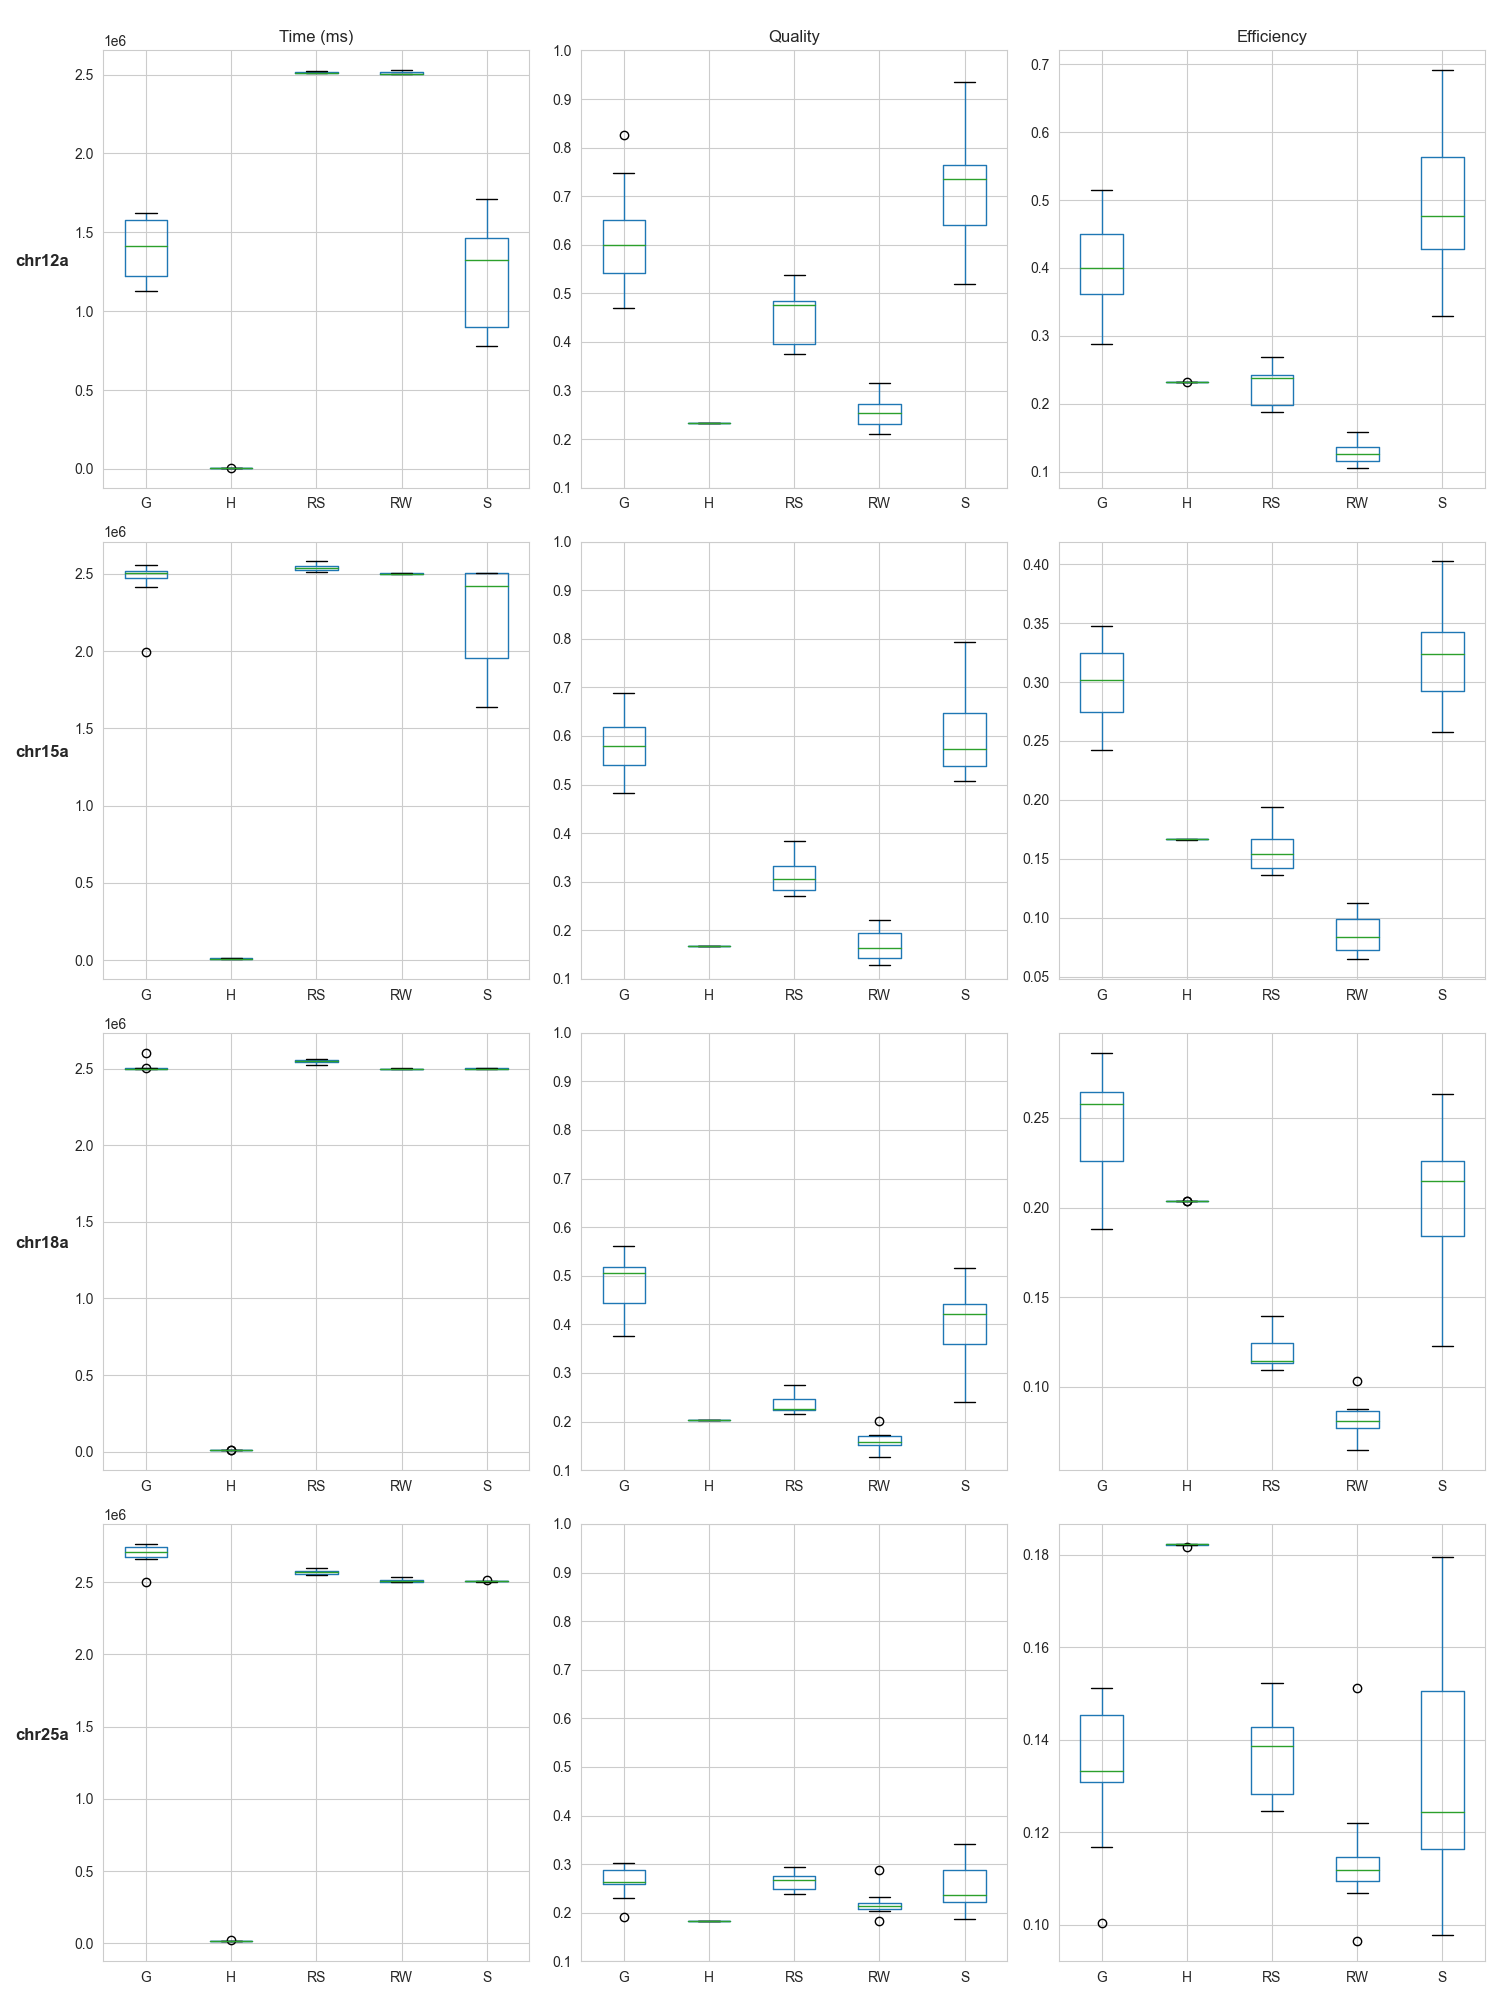
\includegraphics[width=1.0\textwidth]{pics/time_quality_efficiency_box_plots}
    \caption{Comparison of algorithms performance}
    \label{fig:1}
\end{figure}

\pagebreak

In Figure~\ref{fig:2}, the number of algorithmic steps (changes to the current solution) is depicted on the right side of the plot,
while the number of evaluated (fully or partially) solutions is shown on the left side.
The number of algorithmic steps is higher for the Greedy Algorithm compared to the Steepest Algorithm.
This disparity arises because the Greedy Algorithm continuously modifies the solution to maximize improvement,
while the Steepest Algorithm evaluates all possible neighbors before selecting the best one, resulting in less frequent solution changes.
Conversely, the number of evaluated solutions is lowest for the Random Search algorithm.
This is because Random Search requires full evaluation of each solution to assess its quality, which is more time-consuming compared to partial evaluation.
Additionally, there is a cost associated with updating the best encountered solution,
which requires copying the entire solution—a process that is not necessary for algorithms like Greedy and Steepest, where only two elements are swapped.

The Greedy algorithm conducts fewer evaluations than the Steepest and Random Walk algorithms because it does not allow for non-improving moves
and can terminate earlier.
On the other hand, Random Walk and Steepest algorithms perform a similar number of evaluations
since they allow for non-improving moves and conduct partial evaluations at each step.


\begin{figure}[H]
    \centering
    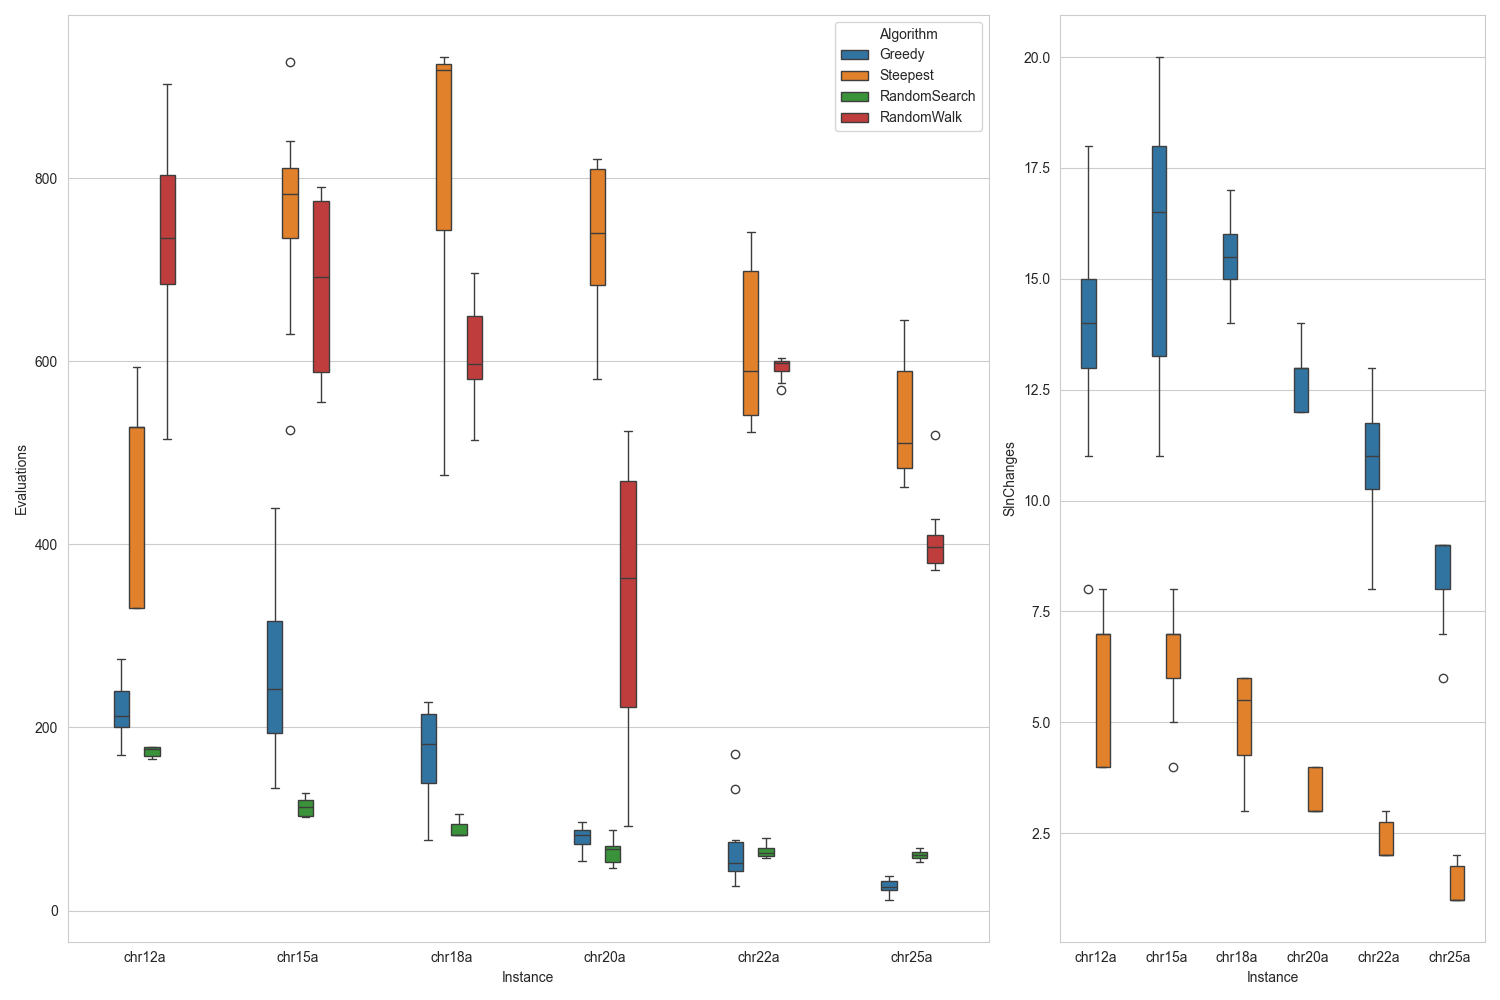
\includegraphics[width=1.0\textwidth]{pics/evaluations_sln_changes_box_plot}
    \caption{Number of algorithmic steps and evaluated solutions}
    \label{fig:2}
\end{figure}

\subsection{Initial solution influence}\label{subsec:initial-solution-influence2}
Figure~\ref{fig:3} illustrates the relationship between the quality of the solution and the quality of the initial solution.
The test was conducted for the Greedy and Steepest algorithms across three instances: chr12a, chr20a, and lipa20a.
Interestingly, the quality of the solution does not appear to depend on the quality of the initial solution.
This observation is consistent across both algorithms and all instances, as evidenced by the correlation coefficient, which is close to zero.


\begin{figure}[H]
    \centering
    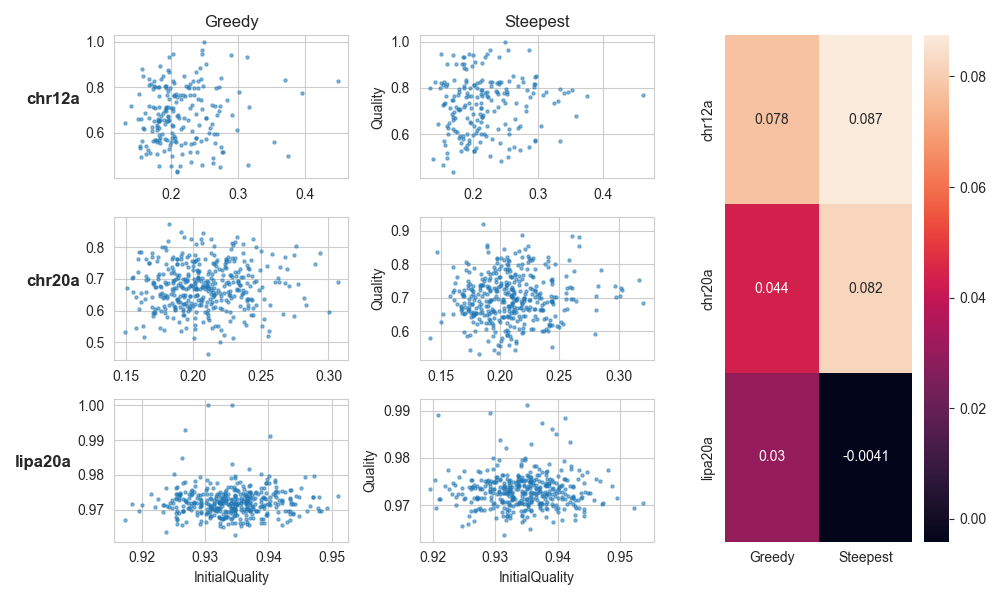
\includegraphics[width=1.0\textwidth]{pics/initial_quality_correlation_heatmap}
    \caption{Quality of the solution vs quality of the initial solution}
    \label{fig:3}
\end{figure}

\subsection{Algorithm performance over subsequent runs}\label{subsec:algorithm-performance-over-subsequent-runs}
Figure~\ref{fig:4} presents the average and lowest cost of the solution for the Greedy and Steepest algorithms obtained up to the $i$-th run.
It is noticeable that the average cost of the solution remains relatively stable after the first 50 runs.
The most significant decrease in cost occurs within the initial 10 runs.
Subsequent reductions in cost occur intermittently, with noticeable decreases observed after approximately 100 to 300 runs, depending on the instance.
Therefore, it is advisable to run the algorithm for at least 10 or 20 iterations to observe substantial improvements in solution quality.

\begin{figure}[H]
    \centering
    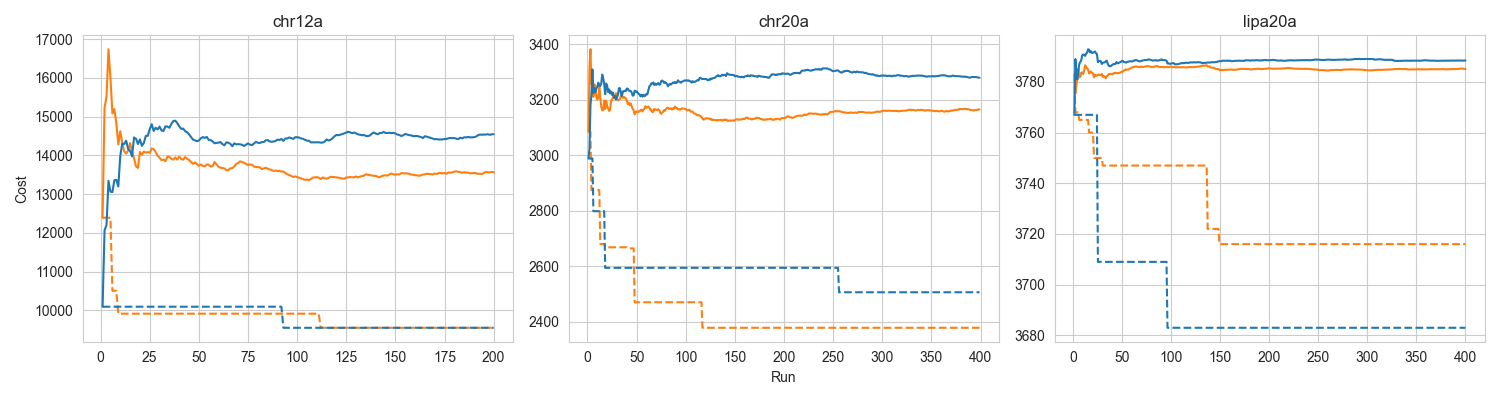
\includegraphics[width=1.0\textwidth]{pics/initial_quality_cost_so_far}
    \caption{Average and lowest cost of the solution}
    \label{fig:4}
\end{figure}

\subsection{Distance from optimal solution in decision space}\label{subsec:distance-from-optimal-solution-in-decision-space}
The correlation between the quality of the solution and the distance in decision space from the optimal solution,
calculated as the number of elements that differ between the permutation representing the solution and the optimal permutation,
is depicted in Table~\ref{tab:1} for two instances, tai12b and tai100b.
Corresponding scatter plots are provided in Figure~\ref{fig:5}.
For both instances, tai12b and tai100b, the correlation is negative,
indicating that the quality of the solution tends to decrease as the distance from the optimal solution increases.
However, the correlation is not significant, suggesting that local minima are distributed across the decision space.

\begin{table}[H]
    \centering
    \begin{tabular}{|c|c|c|}
        \hline
        Instance & Algorithm & Correlation \\
        \hline
        tai12b & Greedy & -0.46 \\
        tai12b & Steepest & -0.51 \\
        tai100b & Greedy & -0.63 \\
        tai100b & Steepest & -0.53 \\
        \hline
    \end{tabular}
    \caption{Correlation between the quality of the solution and the distance in decision space from optimal solution}
    \label{tab:1}
\end{table}

\begin{figure}[H]
    \centering
    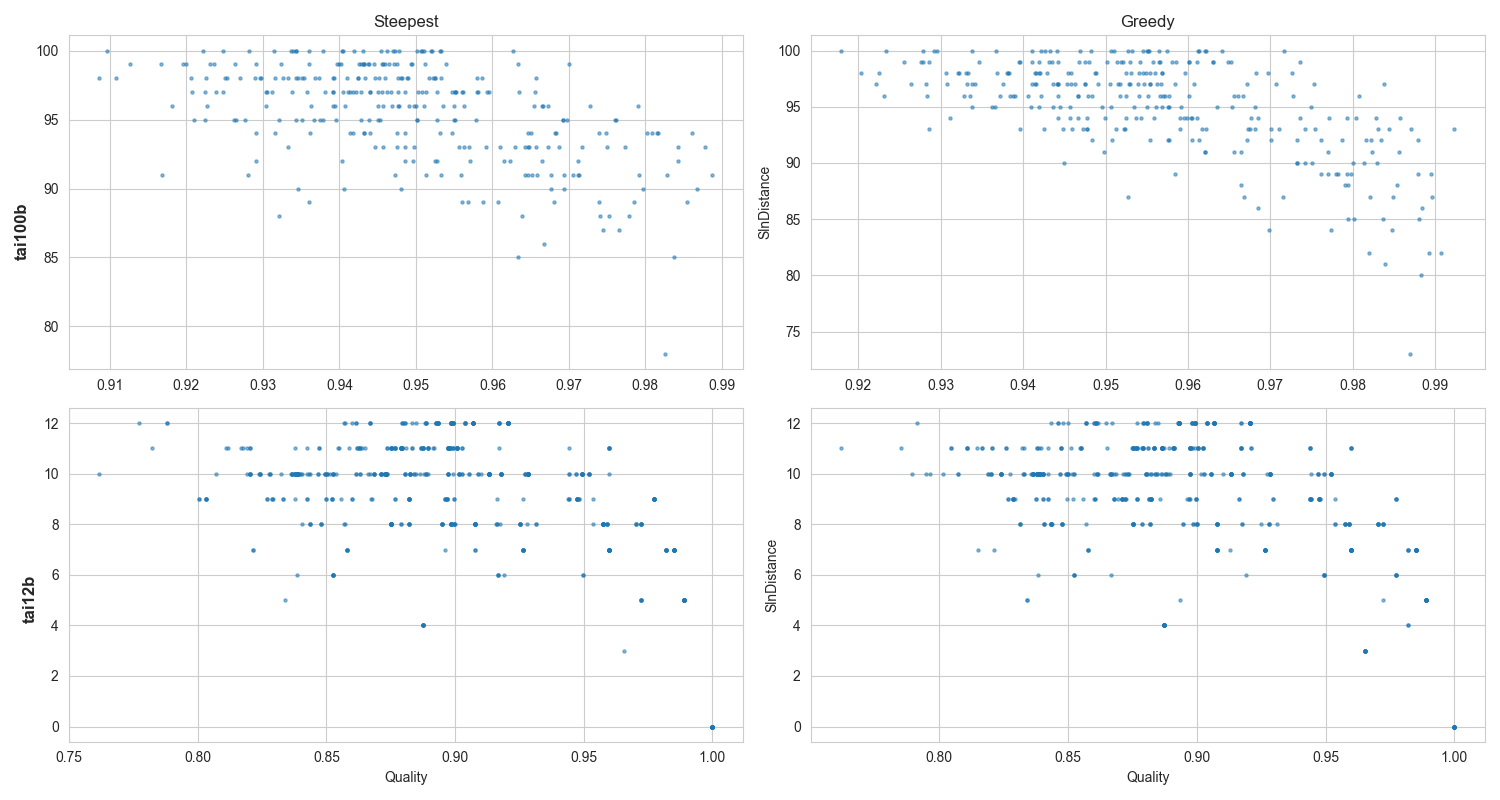
\includegraphics[width=1.0\textwidth]{pics/repetitions_quality_distance_scatter}
    \caption{Quality of the solution vs distance from optimal solution}
    \label{fig:5}
\end{figure}

\section{Conclusions}\label{sec:conclusions}
The Quadratic Assignment Problem (QAP) poses a significant challenge in combinatorial optimization, finding applications across diverse fields.
This study evaluated the performance of five algorithms - Heuristic, Steepest, Greedy, Random Walk, and Random Search - on a range of QAP instances.
The results demonstrate that the Greedy and Steepest algorithms consistently outperform the Random Walk and Random Search algorithms in terms of solution quality.
Although the Heuristic algorithm yields suboptimal solutions,
its advantage lies in its speed, making it suitable for less challenging instances prioritizing efficiency.
Both the Greedy and Steepest algorithms emerge as top performers in solution quality.
However, the choice between them should consider specific problem requirements, as the difference in performance is not substantial.
Conversely, the Random Walk and Random Search algorithms deliver poor results, with solution quality deteriorating as instance difficulty increases.
Variations in the number of algorithmic steps and evaluated solutions are observed among algorithms,
with the Greedy algorithm conducting fewer evaluations compared to Steepest and Random Walk algorithms.
Furthermore, for the Greedy and Steepest algorithms, the quality of the solution is found to be independent of the initial solution quality.
The stability of average and lowest solution costs after a certain number of runs suggests the benefit of running the algorithm for at least 10 to 20 iterations.
Regarding the relationship between solution quality and distance from the optimal solution,
a negative correlation is observed for both instances tai12b and tai100b.
This indicates that solution quality tends to decrease as the distance from the optimal solution increases.
However, the lack of significance in the correlation implies that local minima are scattered throughout the decision space.

In summary, while the Greedy and Steepest algorithms exhibit superior performance,
careful consideration of algorithmic characteristics and problem requirements is essential for algorithm selection.
Further research could explore algorithmic enhancements and strategies for addressing challenges posed by local minima.

\section{Future Work}\label{sec:future-work}
In future studies, enhancing the heuristic algorithm for the Quadratic Assignment Problem (QAP) by considering pairs of rows in each assignment step
could be promising.
Instead of assigning the highest sum row in matrix \(A\) to the lowest sum row in matrix \(B\),
we can explore assigning the two highest sum rows in \(A\) to the two lowest sum rows in \(B\).
This approach aims to minimize the total cost by carefully selecting pairs of rows that offer the most favorable assignment options.
Implementing this refined assignment strategy within the heuristic algorithm would involve adapting the assignment mechanism to evaluate pairs of rows
from matrices \(A\) and \(B\) systematically.
By considering multiple potential assignments simultaneously, the algorithm could explore a broader range of possible solutions
and potentially identify more favorable combinations leading to improved solution quality.

However, it's important to note that this enhanced approach may require significantly more computational power,
resulting in slightly longer execution times.
The increased complexity of evaluating pairs of rows in each assignment step could lead to a higher computational burden,
particularly for larger QAP instances.

Evaluating the performance of this enhanced heuristic algorithm across various QAP instances
would be essential to assess its effectiveness and efficiency.

In summary, exploring the idea of considering pairs of rows in each assignment step represents a promising avenue for advancing
this heuristic algorithm and enhancing its performance in solving the Quadratic Assignment Problem.

\pagebreak
% \begin{multicols}{2}

% \end{multicols}
% \begin{figure} % a figure appears in the source before the first reference to it -- a useful rule of thumb
% \begin{center}
% 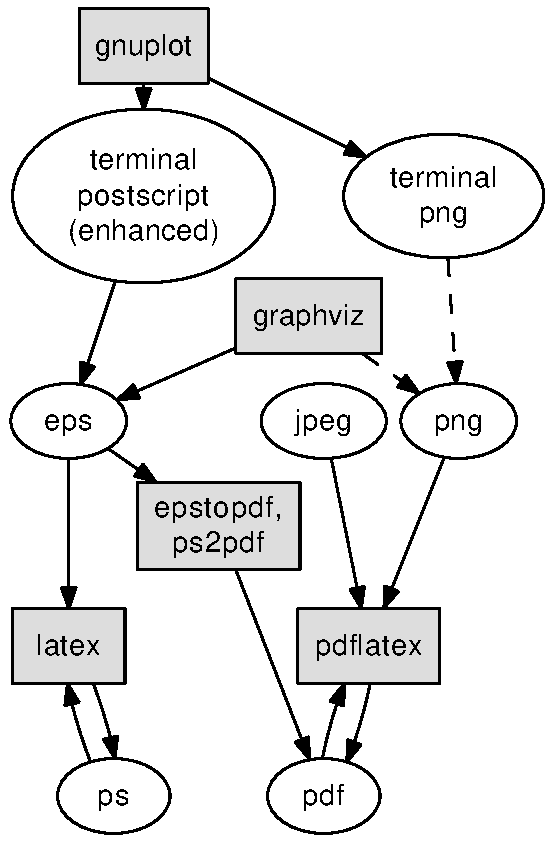
\includegraphics[width=0.4\textwidth]{rys_graf.pdf}
% \end{center}
% \caption{Example diagram from the \emph{graphviz} program, which is a tool that automatically produces diagram layouts~\cite{graphviz}. Remember that wherever possible, we use vector graphics -- avoid embedding bitmaps in the document. In some cases, the use of bitmaps is justified (for quick on-screen previews or for extremely complex graphics containing, for example, hundreds of thousands of objects). The differences in raster and vector graphics are discussed (in Polish) in~\url{https://www.youtube.com/watch?v=_98SDNIpm24}.}
% \label{fig:schemat}
% \end{figure}


% This is a sample text in LaTeX. Read it carefully (the content, its source and the \%comments) and use the \texttt{*.tex} source as a report template -- it shows how to

% \begin{tightlist}
% \item insert a diagram created by graphviz (Fig.~\ref{fig:schemat}),
% \item insert a plot created by gnuplot (Fig.~\ref{fig:3d}) and matplotlib (Fig.~\ref{fig:matplotlib}),
% \item cite bibliography formatted by bibtex~\cite{LS-lectures,Goldberg-2002},
% \item refer to figures, references and parts of the report (for example, Sect.~\ref{sec:typografia}),
% \item as well as to equations: note, usually we do not write the word ``equation'', we just write it like this: In~\eqref{eq:mysterious-equation}, a surprising property of some mathematical transformations is shown.
% \end{tightlist}


% \begin{equation}
% \label{eq:mysterious-equation}
% e^{i \pi} = -1 = \sqrt {-1} \sqrt {-1} = \sqrt {-1 \cdot -1} = \sqrt 1 = 1
% \end{equation}





%\section{The characteristics of a good report}
%
%A good report
%\begin{tightlist}
%\item allows the reader to independently reproduce the experiment (from data to results),
%\item contains no ambiguities,
%\item presents conclusions organized from general to specific,
%\item cites the literature in the text,
%\item does not include oversized listings,
%\item clearly presents the results -- usually using plots,
%\item shows any numerical data with the correct number of significant figures,
%\item is concise and aesthetic.
%\end{tightlist}
%
%\noindent An important rule of thumb when writing any report, thesis or paper is that the accompanying data, figures and plots should always have some sort of associated conclusions -- to avoid overwhelming the reader with tables and graphs that they themselves must interpret, since they could not find the appropriate conclusions in the text. The evaluators of the reports evaluate the conclusions, not the fact that the computations were carried out and proved by the included results. In particular, including just the results and plots without explicitly written conclusions and interpretations is almost worthless from the evaluation point of view -- because it says almost nothing about the author's expertise and reasoning. If such a report, rich in results but deficient in conclusions, were by contrast read by an amateur who wanted to learn something new -- they would hardly learn much. So there must be a balance in the report: the included results must have corresponding conclusions and must be commented on in some way, and the written conclusions must be explicitly supported by the included data (e.g., plots).





%\subsection{Typography}
%\label{sec:typografia}
%
%Remember about the difference between a hyphen\footnote{Read Wikipedia's description of the entry ``Hyphen''.} and a dash -- as well as about citing any source material in the relevant places~\cite{WikiDash}. Cite a specific page, not the general address of the website. Write double quotation marks using ``the method of two marks''. Accordingly, with single quotation marks we distinguish between `opening and closing' ones.
%
%For spell-checking the\ .tex file directly, there is, among others, the \emph{aspell} program. It understands various text encodings and has built-in filters for html and other popular formats. With these filters, it omits keywords specific to a given file format, and only analyzes the actual text. % the backslash before the space cues LaTeX to use a regular space (rather than a widened space). In this case, it is not necessary, but in general, this is how we indicate that any period before a space is not the end of a sentence (such an indication is sometimes needed, because LaTeX by default makes wider spaces after all periods assuming that periods separate sentences -- which is almost always right).
%
%
%
%
%
%
%
%\section{Plots}
%
%\noindent For processing text result files and drawing plots, Python accompanied by the matplotlib library is excellent. They are definitely worth learning! Before you prepare a plot, you can watch tips (in Polish) on creating plots and follow them -- how to make a legible and professional plot:~\url{https://www.youtube.com/watch?v=pfSgcsQ2Mtk}. % the tilde is the non-breaking space -- it sticks adjacent words together.
%
%
%\begin{figure}
%\begin{center}
%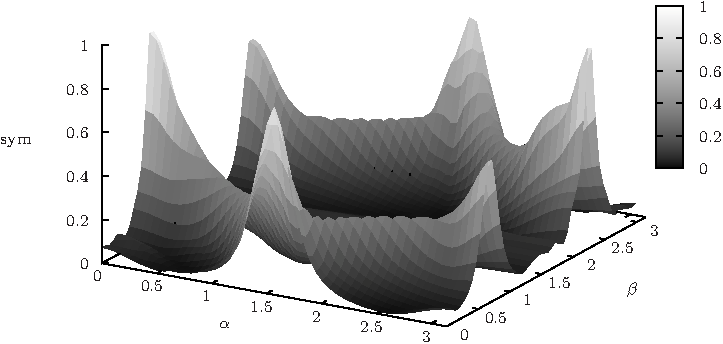
\includegraphics[width=0.9\textwidth]{rys_wykres3d.pdf}
%\end{center}
%\caption{A sample plot, this one produced by the \texttt{gnuplot} program.}
%\label{fig:3d}
%\end{figure}
%
%
%\begin{figure}
%\begin{center}
%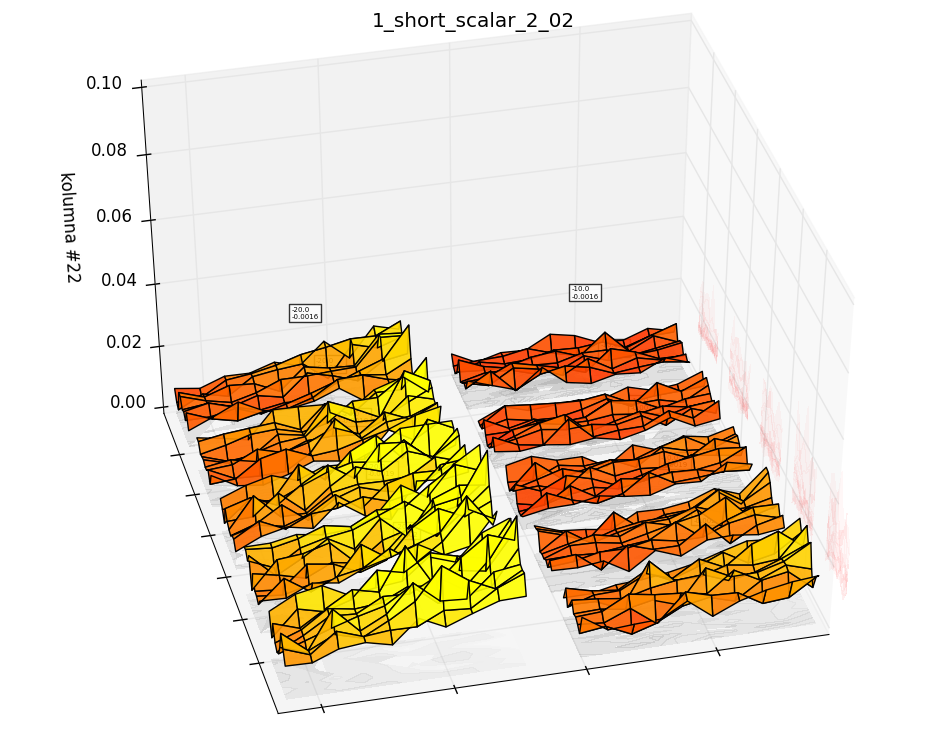
\includegraphics[width=0.48\textwidth]{rys_short_scalar_2_02.png}\hfill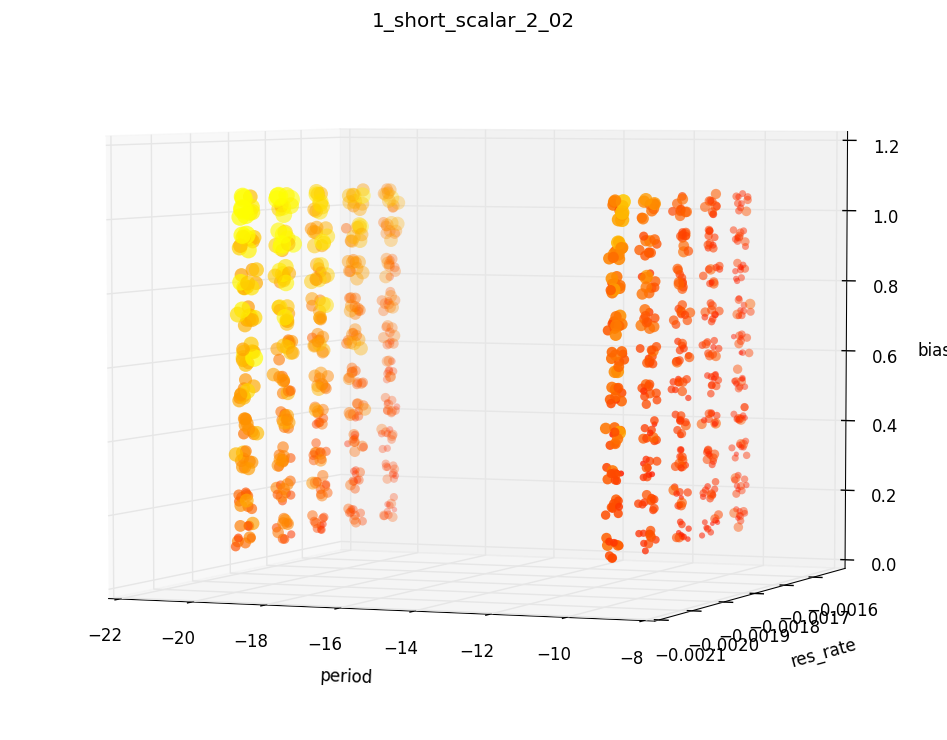
\includegraphics[width=0.48\textwidth]{rys_short_scalar_2_02-kulki.png}
%\end{center}
%\caption{A sample visualization in \texttt{Python}+\texttt{matplotlib}; here, 5D data shown in two ways in 3D. What is wrong with this figure? Bitmaps are used (incorrectly -- should be vector graphics), and the plots here are too small (illegible).}
%\label{fig:matplotlib}
%\end{figure}
%
%\clearpage % let LaTeX put pending figures right here -- this command "releases" the accumulated content, which is useful if you have placed a lot of images, much more than text -- so they do not appear at the end of the document.
%
%
%
%
%
%\section{In closing}
%
%And now something extra. As you have read this entire text source, handle one inconspicuous sentence: \url{http://www.mooncoder.com/latex-challenge.html} %and never again forget what is the difference between hyphens and dashes!


%%%%%%%%%%%%%%%% references %%%%%%%%%%%%%%%%

%\bibliography{biblio}
%\bibliographystyle{plainurl}

\end{document}
